% include the figures path relative to the master file
\graphicspath{ {./content/results/figures/} }

\section{Results} 
A lack of public data in order to perform fair comparison between methodologies is a recurrent problem in medical imaging.
\ac{bus} images are no exception \cite{Cheng:2009p10580}. 
Therefore segmentation can only be compared for the lesions segmentation case, and only against the results reported in the bibliography.

\Cref{fig:surveyResults} compares our segmentation strategy against the state-of-the-art assuming the following limitations:
(a) the other methodologies' performance has been collected from the literature. 
(b) Since all the segmentation results are reported using different metrics, those have been translated to \ac{aov} as a common evaluation metric.
(c) Evaluation datasets not only differ in image acquisition but also their sizes suffer a large variation. 

Every methodology from the literature is represented in a 
uncommon dataset, different levels of user assistance to perform the segmentation, 

A fair comparison with other segmentation methodologies is impossible. 
Trying to assess a novel segmentation strategy for delineating tissues in \ac{bus} images is a challenge by itself.
Cheng:2009p10580,
However, the lack of a common dataset to test all the methodologies with makes impossible a fair comparison between methods. This is easily observed when comparing the segmentation results reported from automatic methodologies those outperform manual segmentations done by trained expert radiologists. 

Pons et al.~\cite{gerard2013} analyzed the inter- and intra-observer variability of manual segmentations of breast lesions in \ac{us} images. In the experiment, a subset of 50 images is segmented by an expert radiologist and 5 expert biomedical engineers with deep knowledge of a breast lesion appearance in \ac{us} data. The experiment reported an \ac{aov} rate between $0.8$ and $0.852$ for the 6 actors. This demonstrates the large variability between \ac{gt} delineations; a fact that needs to be taken into account in order to draw proper conclusions about the performance of a segmentation methodology. However, having multiple \ac{gt} delineations to better assess the segmentations performance is not always possible. When possible, several strategies have been used to incorporate such information.

lthough the new segmentation technique achieves results are comparable only to some of the results published in the bibliography (see fig.~\ref{fig:surveyComp}), the proposed methodology has large room for improvement compared to our previous proposal which was pretty tuned up already (see section~\ref{sec:method:previousWork}). In this last affirmation it needs to be taken into account such methodologies against the rest of the methodologies in the literature is unfeasible due to the lacking common dataset. 



In order to facilitate the comparison between the proposed methodology and the methodologies reviewed in chapter~\ref{chapter:survey}, despite the bias of being tested in different datasets, the figure~\ref{fig:performanceComparison}a is replicated here in figure~\ref{fig:surveyComp} this time showing an extra ring in black at $0.623$ representing the best performance in fig.~\ref{fig:quantResultsAOV}a, so that it can be easily compared to the previously reviewed methodologies.


\begin{figure}[h]
  \centering
  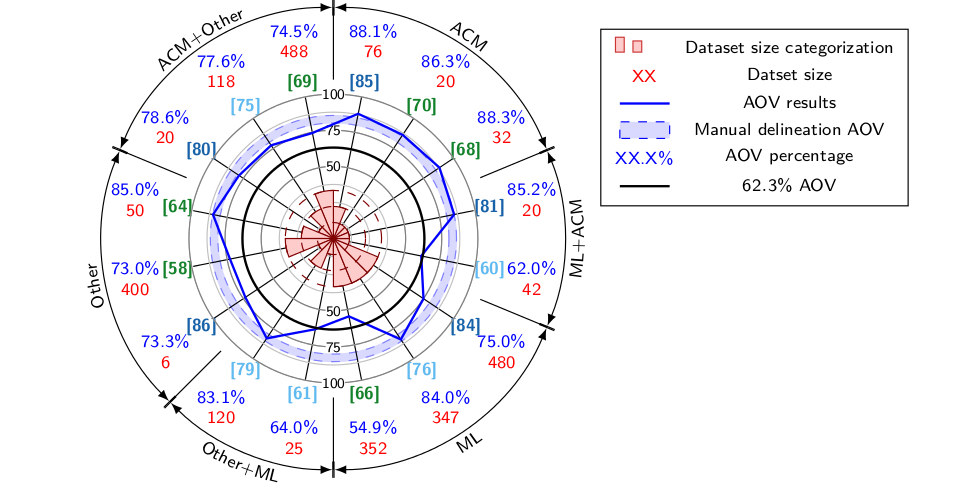
\includegraphics[width=0.8\linewidth]{results}
  \caption{Quantitative AOV results}
  \label{fig:surveyResults}
\end{figure}
%%% Local Variables: 
%%% mode: latex
%%% TeX-master: "../../master.tex"
